
%(BEGIN_QUESTION)
% Copyright 2011, Tony R. Kuphaldt, released under the Creative Commons Attribution License (v 1.0)
% This means you may do almost anything with this work of mine, so long as you give me proper credit

Suppose a DP transmitter with a calibrated range of -30 to +30 inches water column (4 to 20 mA output) is subjected to the following pressure:

$$\includegraphics[width=15.5cm]{i03464x01.eps}$$

Calculate the voltage dropped by the resistor:

\vskip 10pt

$V$ = \underbar{\hskip 50pt} volts (no transmitter error)

\vskip 30pt

Now suppose the transmitter has a ``zero shift'' error of +2\% of span (i.e. its output signal is 2\% of span greater than it should be at all points along its calibrated range).  Re-calculate the voltage dropped by the resistor:

\vskip 10pt

$V$ = \underbar{\hskip 50pt} volts (with +2\% transmitter error)

\underbar{file i03464}
%(END_QUESTION)





%(BEGIN_ANSWER)

\noindent
5 points for each answer:

\vskip 10pt

$V$ = \underbar{\bf 6.16} volts (no transmitter error)

$V$ = \underbar{\bf 6.266} volts (with +2\% transmitter error)

%(END_ANSWER)





%(BEGIN_NOTES)

{\bf This question is intended for exams only and not worksheets!}.

%(END_NOTES)


